\documentclass[10pt]{article}
\usepackage[a4paper, total={6in,9in}]{geometry}
\usepackage[parfill]{parskip}    	
\usepackage{graphicx,caption,fancyhdr,xcolor,pdfpages,setspace}
\usepackage{minted}
\usepackage{xcolor}
\usepackage[
        colorlinks = true,
        allcolors  = darkgray
]{hyperref}



\newcommand{\wrt}[1]{\mathrm{d}#1}


\setlength{\fboxsep}{0.5em}



\urlstyle{same}
\renewcommand{\footnoterule} % Push footnotes to the bottom of the page
	{\vfill\kern -3pt \hrule width 0.4\columnwidth \kern 2.6pt}

\makeatletter
\title{Digital Design with HDL Lab3}
\let\Title\@title
\author{Y3862181 \& Y3899129}
\let\Author\@author
\date{Autumn Term, 2022}
\let\Date\@date
\makeatother


\fancypagestyle{content}{
    \renewcommand{\headrulewidth}{0.4pt}
    \renewcommand{\footrulewidth}{0.4pt}
    \setlength{\headheight}{15pt}
    
	\fancyhf{}
	\fancyhead[L]{\Author}
	\fancyhead[R]{\Title}
	\fancyfoot[L]{\Date}
	\fancyfoot[R]{\thepage}
}
\onehalfspacing

\begin{document}
\begin{titlepage}
\centering
{\Huge Lab Report 3}

\vspace{3cm}

{\LARGE \textbf{Digital Design with HDL}}

\vspace{3cm}

{\huge Y3862181 \& Y3899129}

\vspace{2cm}


{\large Autumn Term, 2022}
\vfill

{\itshape University of York}
\end{titlepage}

\tableofcontents
\newpage

\pagestyle{content}
\section{Introduction}
This lab focuses on using memory components and implementing circuits that involve a Finite State Machine (FSM).

Part A exposes the implementation of a Fibonacci generator using predefined values stored in a ROM array, as well as covers some prerequisite theory regarding memory in digital electronics.

Part B shows the implementation of a circuit with almost the same behaviour as in part A, except that the Fibonacci numbers are computed in real time using a FSM.

\newpage


\section{Task A: Implementation of Memories}

\subsection{Implementation of an Asynchronous ROM \texttt{(async\_rom.vhd)}}

\begin{minted}{vhdl}
library IEEE;
use IEEE.STD_LOGIC_1164.ALL;
use IEEE.NUMERIC_STD.all;

-- Implementation of an asynchronous ROM that stores 
-- Fibonacci numbers up to 233, which is the 14th number

entity async_rom is
    Port ( address  : in UNSIGNED (3 downto 0);
           data_out : out STD_LOGIC_VECTOR (7 downto 0));
end async_rom;

architecture arch of async_rom is

-- The ROM_array stores the numbers of the Fibonacci sequence 
-- as a type STD_LOGIC_VECTOR
type ROM_array is array (0 to 13) of std_logic_vector(7 downto 0);
    constant Content: ROM_array :=  (
        0  => x"00",
        1  => x"01",
        2  => x"01",
        3  => x"02",
        4  => x"03",
        5  => x"05",
        6  => x"08",
        7  => x"0d",
        8  => x"15",
        9  => x"22",
        10 => x"37",
        11 => x"59",
        12 => x"90",
        13 => x"e9",
    others => B"00000000"); -- Returned value when an illegal address is provided
begin
    -- The index of the array should be of type integer.
    data_out <= Content(to_integer(address)); 

end arch;
\end{minted}
\newpage


\subsection{Implementation of a Synchronous Counter \texttt{(sync\_counter.vhd)}}

\begin{minted}{vhdl}
library IEEE;
use IEEE.STD_LOGIC_1164.ALL;
use IEEE.NUMERIC_STD.all;

-- Implementation of a synchronous counter with reset and enable, 
-- used to generate the indices of the Fibonacci numbers
-- It counts until number 13 is reached

entity sync_counter is
    Port ( clk : in STD_LOGIC; -- Clock input signal
           rst : in STD_LOGIC; -- Reset signal
           en  : in STD_LOGIC; -- Count enable signal
           count_out : out UNSIGNED (3 downto 0)); -- Output of the counter
end sync_counter;

architecture Behavioral of sync_counter is

-- Internal counter bus
signal count_internal : UNSIGNED (3 downto 0);

begin

-- The process of the counter, which implements
-- the synchronous reset and enable
sync_counter: process (clk)
begin
    if ( rising_edge ( clk ) ) then
        if ( rst = '1' ) then
            count_internal <= ( others => '0' );
        elsif ( en = '1' ) then
            if ( count_internal = 13 ) then
                count_internal <= ( others => '0' );
            else
                count_internal <= ( count_internal + 1 );
            end if;
        end if;
    end if;
end process sync_counter;

count_out <= count_internal;  
end Behavioral;
\end{minted}
\newpage

\subsection{Implementation of a Fibonacci Generator \texttt{(fibonacci.vhd)}}
\begin{minted}{vhdl}
library IEEE;
use IEEE.STD_LOGIC_1164.ALL;
use IEEE.NUMERIC_STD.all;

-- Implementation of an 8-bit Fibonacci generator

entity fibonacci is
    Port ( clk        : in STD_LOGIC; -- input for the system clock
           en_button  : in STD_LOGIC; -- Unfiltered enable button
           rst_button : in STD_LOGIC; -- Unfiltered reset button
           fib_out    : out STD_LOGIC_VECTOR (7 downto 0)); -- Fibonacci output
end fibonacci;

architecture Behavioral of fibonacci is

signal deb_rst_button : STD_LOGIC; -- Filtered signal from the reset button
signal deb_en_button  : STD_LOGIC; -- Filtered signal from the enable button
signal address        : UNSIGNED (3 downto 0); -- Address of the Fibonacci number

begin

-- Block to filter the signal from the reset button and implement an 
-- edge detection
DEBOUNCE_RST: entity work.DEBOUNCE
PORT MAP (
    clk => clk,
    sig => rst_button,
    deb_sig => deb_rst_button
);

-- Block to filter the signal from the enable button and implement an
-- edge detection
DEBOUNCE_EN: entity work.DEBOUNCE
PORT MAP (
    clk => clk,
    sig => en_button,
    deb_sig => deb_en_button
);
\end{minted}
\newpage
\begin{minted}{vhdl}
-- Block to count from 0 to 13 using the filtered signals for the
-- enable and the reset. The 13th index of the Fibonacci sequence
-- is the largest number that could fit in 8-bits
COUNTER: entity work.sync_counter
PORT MAP (
    clk => clk,
    en  => deb_en_button,
    rst => deb_rst_button,
    count_out => address
);

-- Block to map the index generated from the counter to its 
-- corresponding Fibonacci number
FIB_ROM: entity work.async_rom
PORT MAP (
    address => address,
    data_out => fib_out
);

end Behavioral;
\end{minted}
\newpage

\subsection{Testing the Fibonacci Generator \texttt{(fibonacci\_tb.vhd)}}

\begin{minted}{vhdl}
library IEEE;
use IEEE.STD_LOGIC_1164.ALL;

-- Testbench to verify the correct operation of the Fibonacci Generator

entity fibonacci_tb is
end fibonacci_tb;

architecture Behavioral of fibonacci_tb is

constant clk_period : time := 10ns;

signal clk          : STD_LOGIC; -- Clock signal
signal rst_button   : STD_LOGIC; -- Unfiltered reset signal
signal en_button    : STD_LOGIC; -- Unfiltered enable signal
signal fib_out      : STD_LOGIC_VECTOR (7 downto 0); -- Fibonacci Output

begin

-- Process to generate the clock signal
clk_process : process
begin
    clk <= '0';
    wait for clk_period / 2;
    clk <= '1';
    wait for clk_period / 2;
end process;

UUT: entity work.fibonacci
    PORT MAP (
        clk        => clk,
        rst_button => rst_button,
        en_button  => en_button,
        fib_out    => fib_out
    );
\end{minted}
\newpage
\begin{minted}{vhdl}
-- Testing strategy: firstly, initial values are set and a reset procedure
-- is performed. Then, a cycle 0 to 25 drives the next state input
-- of the controller aiming to verify the correct functionality of the
-- Fibonacci numbers generation. After that, another reset
-- sequence is performed for confirming that the generator resets correctly,
-- followed by a loop to prove that it is stable after the reset

TEST:   process
begin
    -- Synchronization
    wait for 100ns;
    wait until falling_edge(clk);
    
    -- Set initial values
    rst_button <= '0';
    en_button <= '0';
    wait for clk_period*3;
    
    -- Reset the controller in order to clear the counters
    rst_button <= '1';
    wait for clk_period*3;
    rst_button <= '0';
    wait for clk_period*3;
    
    -- Loop to verify the Fibonacci number generation
    loop_25: for i in 0 to 25 loop
        en_button <= '1';
        wait for clk_period*3;
        en_button <= '0';
        wait for clk_period*3;
    end loop loop_25;

    -- Final reset to test the reset functionality
    rst_button <= '1';
    wait for clk_period*3;
    rst_button <= '0';
    wait for clk_period*3;
\end{minted}
\newpage
\begin{minted}{vhdl}
    -- Loop to prove that the circuit works correctly after the reset
    loop_5: for i in 0 to 5 loop
        en_button <= '1';
        wait for clk_period*3;
        en_button <= '0';
        wait for clk_period*3;
    end loop loop_5;
    
    wait;
end process;

end Behavioral;
\end{minted}
\newpage
\subsection{Simulation}
From the timing diagram in \autoref{fig:sim_a_beg}, it can be observed that at time zero all of the inputs and the output of the internal counter are in an undefined state. In addition, the output of the Fibonacci controller is displaying 0, because this is the default state implemented in the Fibonacci ROM. After the initial 100ns the inputs are set to an initial value (logic zero) for both the reset and enable lines.
Following that, a reset signal occurs and it can be seen that on the second rising edge of the clock, the debouncer generates the internal reset signal (“rst\_deb”), which clears the internal counter from undefined to zero. Furthermore, a steady sequence of enable signals is generated, which increments the counter and the Fibonacci number generation. The choice of radices for both fib\_out and count\_out is in decimal for clarification purposes.
\begin{figure}[ht]
    \centering
    \fbox{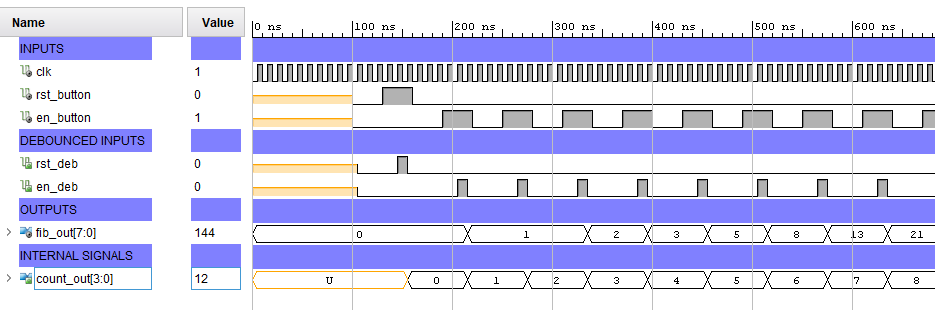
\includegraphics[width=0.9 \textwidth]{sim_a_beg.png}}
    \caption{Initialisation stage of the Fibonacci generator}
    \label{fig:sim_a_beg}
\end{figure}

The timing diagram in \autoref{fig:sim_a_goes_to_0} shows that when the final Fibonacci number is generated (233 with index 13), the generator rolls over and starts generating the Fibonacci sequence from zero again.
\begin{figure}[ht]
    \centering
    \fbox{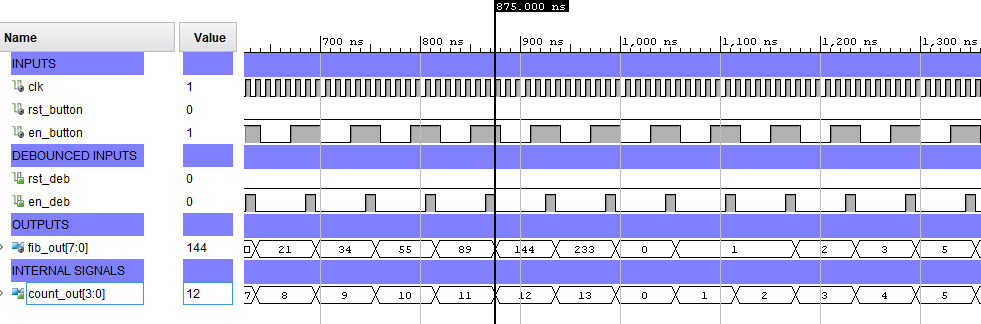
\includegraphics[width=0.9 \textwidth]{sim_a_goes_to_0.png}}
    \caption{Fibonacci sequence continues until the Fibonacci generator goes to 0}
    \label{fig:sim_a_goes_to_0}
\end{figure}
\newpage

 \autoref{fig:sim_a_mid_reset} shows that a second reset was performed in order to prove that the reset works correctly.
\begin{figure}[ht]
    \centering
    \fbox{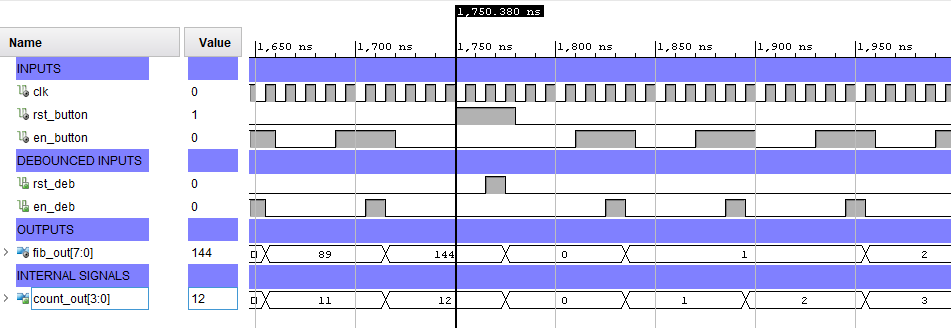
\includegraphics[width=0.9 \textwidth]{sim_a_mid_reset.png}}
    \caption{Reset behaviour of the Fibonacci generator}
    \label{fig:sim_a_mid_reset}
\end{figure}
\newpage



\subsection{RTL Statistics}
In this section of the lab, the 8-bit Fibonacci generator was implemented successfully and displayed as expected in both
the RTL component statistics and the RTL hierarchical component statistics.
\begin{minted}{text}
---------------------------------------------------------------------------------
Start RTL Component Statistics 
---------------------------------------------------------------------------------
Detailed RTL Component Info : 
+---Adders : 
	   2 Input      4 Bit       Adders := 1     
+---Registers : 
	                4 Bit    Registers := 1     
	                1 Bit    Registers := 6     
+---Muxes : 
	   2 Input      4 Bit        Muxes := 1     
---------------------------------------------------------------------------------
Finished RTL Component Statistics 
---------------------------------------------------------------------------------
---------------------------------------------------------------------------------
Start RTL Hierarchical Component Statistics 
---------------------------------------------------------------------------------
Hierarchical RTL Component report 
Module DEBOUNCE 
Detailed RTL Component Info : 
+---Registers : 
	                1 Bit    Registers := 3     
Module sync_counter 
Detailed RTL Component Info : 
+---Adders : 
	   2 Input      4 Bit       Adders := 1     
+---Registers : 
	                4 Bit    Registers := 1     
+---Muxes : 
	   2 Input      4 Bit        Muxes := 1     
---------------------------------------------------------------------------------
Finished RTL Hierarchical Component Statistics
---------------------------------------------------------------------------------
\end{minted}
\newpage

\subsection{Schematic}

\autoref{fig:fibonacci_schematic} presents the top level schematic of the Fibonacci generator. In other words, all of the separate VHDL files that were included in the fibonacci.vhd (DEBOUNCE.vhd, sync\_counter.vhd and async\_rom.vhd) are shown as their own components.
 \begin{figure}[ht]
    \centering
    \fbox{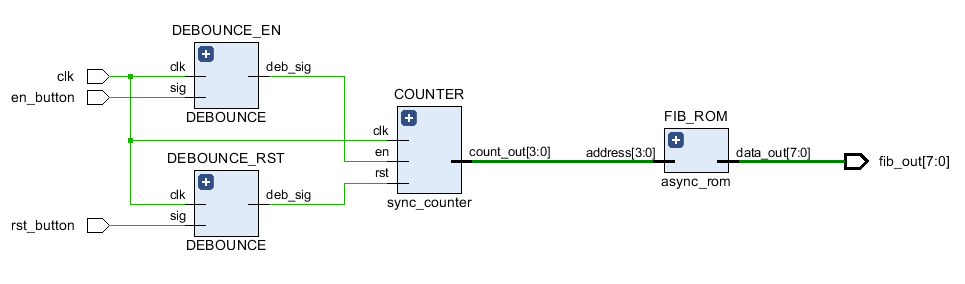
\includegraphics[width=0.9 \textwidth]{fibonacci_schematic.png}}
    \caption{Schematic of the Fibonacci generator}
    \label{fig:fibonacci_schematic}
\end{figure}

From the schematic in \autoref{fig:asynchronous ROM}, it can be seen that it was implemented as a single block of 8-bit ROM, which regarding the VHDL code is exactly an array.
\begin{figure}[ht]
    \centering
    \fbox{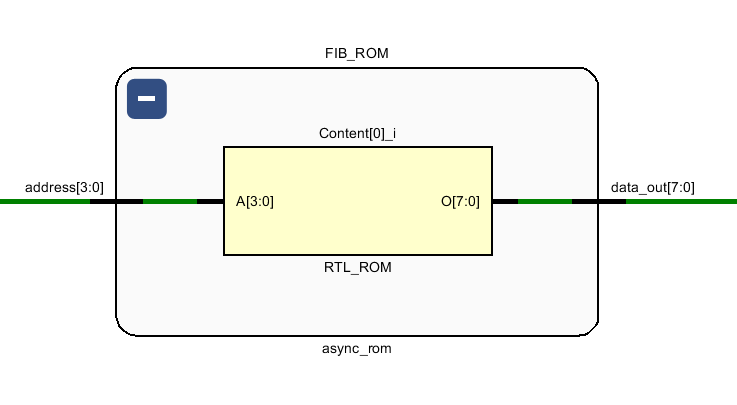
\includegraphics[width=0.9 \textwidth]{fib_rom_schematic.png}}
    \caption{Schematic of the asynchronous ROM}
    \label{fig:asynchronous ROM}
\end{figure}
\newpage

The schematic in \autoref{fig:counter_schematic} is the counter that drives the indices of the Fibonacci numbers, which is a direct interpretation of the VHDL code that produced it. In the code there is an UNSIGNED 4-bit bus which is interpreted as a register with synchronous reset and an enable procedure. The incrementation of the value is interpreted as a feedback with an adder circuit. Which is directly:
\begin{minted}{vhdl}
      count_internal <= ( count_internal + 1 );
\end{minted}
And the if..else... statement is interpreted as a multiplexer.
\begin{figure}[ht]
    \centering
    \fbox{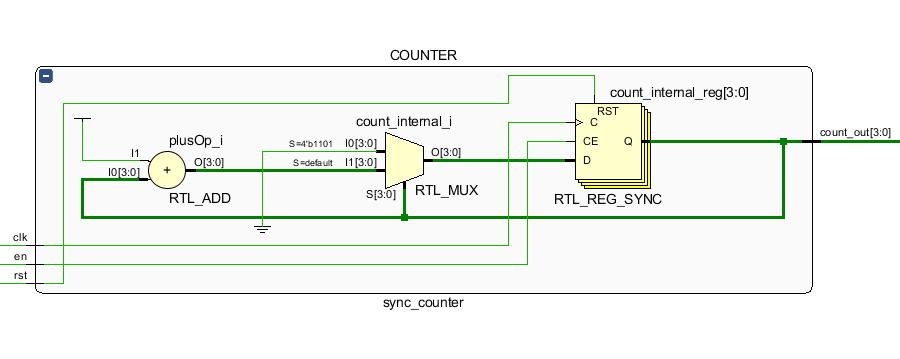
\includegraphics[width=0.9 \textwidth]{counter_schematic.png}}
    \caption{Schematic of the counter}
    \label{fig:counter_schematic}
\end{figure}

The schematic in \autoref{fig:debounce schematic} exhibits the hardware implementation of the debounce circuit (DEBOUNCE.vhd). The implementation uses three separate D-registers, also known as D-type flipflops, and an output word, which collects the data of the outputs of those registers and produces the result of the debounce circuit. This is to be expected, since there were three separate internal STD\_LOGIC\_VECTOR lines in the VHDL file regarding that schematic.

\begin{figure}[ht]
    \centering
    \fbox{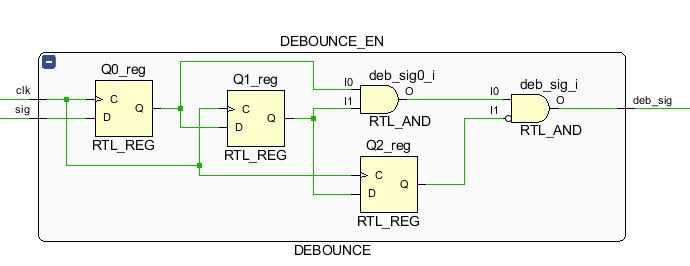
\includegraphics[width=0.9 \textwidth]{deb_schematic.png}}
    \caption{Schematic of the debouncer}
    \label{fig:debounce schematic}
\end{figure}
\newpage

\subsection {Signal to Pin Assignments for the FPGA}
The signal to pin assignments exposed below are used when uploading the design onto the Zedboard Zynq Evaluation and Development Kit (part number xc7z020clg484-1):
\begin{minted}{text}
# Signals to pin assignments

# clock signal -> Y9
set_property PACKAGE_PIN Y9 [get_ports {clk}]
set_property IOSTANDARD LVCMOS18 [get_ports {clk}]

# reset button -> T18
set_property PACKAGE_PIN T18 [get_ports {rst_button}]
set_property IOSTANDARD LVCMOS18 [get_ports {rst_button}]

# enable button -> P16
set_property PACKAGE_PIN P16 [get_ports {en_button}]
set_property IOSTANDARD LVCMOS18 [get_ports {en_button}]

# LED 0 -> T22
set_property PACKAGE_PIN T22 [get_ports {fib_out[0]}]
set_property IOSTANDARD LVCMOS18 [get_ports {fib_out[0]}]

# LED 1 -> T21
set_property PACKAGE_PIN T21 [get_ports {fib_out[1]}]
set_property IOSTANDARD LVCMOS18 [get_ports {fib_out[1]}]

# LED 2 -> U22
set_property PACKAGE_PIN U22 [get_ports {fib_out[2]}]
set_property IOSTANDARD LVCMOS18 [get_ports {fib_out[2]}]

# LED 3 -> U21
set_property PACKAGE_PIN U21 [get_ports {fib_out[3]}]
set_property IOSTANDARD LVCMOS18 [get_ports {fib_out[3]}]

# LED 4 -> V22
set_property PACKAGE_PIN V22 [get_ports {fib_out[4]}]
set_property IOSTANDARD LVCMOS18 [get_ports {fib_out[4]}]

# LED 5 -> W22
set_property PACKAGE_PIN W22 [get_ports {fib_out[5]}]
set_property IOSTANDARD LVCMOS18 [get_ports {fib_out[5]}]
\end{minted}
\newpage
\begin{minted}{text}
# LED 6 -> U19
set_property PACKAGE_PIN U19 [get_ports {fib_out[6]}]
set_property IOSTANDARD LVCMOS18 [get_ports {fib_out[6]}]

# LED 7 -> U14
set_property PACKAGE_PIN U14 [get_ports {fib_out[7]}]
set_property IOSTANDARD LVCMOS18 [get_ports {fib_out[7]}]
\end{minted}
\newpage
\subsection{Prerequisite Theory}
\subsubsection{ROM vs RAM}
ROM stands for Read Only Memory, which suggests that once the memory is programmed it cannot be changed (written or erased). This type of memory is non-volatile, which means that when the device is switched off the memory stored into the ROM will be preserved.
On the other hand, RAM, which stands for Random Access Memory, is a type of memory that can be constantly changed. It supports operations like read, write and erase. A downside of it is that it is volatile, meaning that when the device is powered off the contents of the RAM will be erased.

\subsubsection{Memory Depth vs Memory Width}
Memory depth is a value that describes the total memory capacity of a given device by how many times a data of size "Memory width" can be stored. It can be viewed as the number of memory slots.
Memory width is the capacity of the data that can be stored in every distinct memory address.

In the case of part A of this lab, the ROM that was designed had memory width of 8 bits and memory depth of 14.

\subsubsection{Memory Depth and Address}
Memory depth can't be higher than the number of distinct addresses, but the number of distinct addresses can be bigger than the memory depth.
The biggest memory depth can be observed from:
\begin{equation}
(memory\_depth) = 2^{(address\_width)}
\end{equation}
Equation 1 can be rearranged for calculating address width as a function of memory depth:
\begin{equation}
(address\_width) = \log_2 (memory\_depth)
\end{equation}
For example if a memory device has to store 36 values, then the address width would be:
\[\log_2 (32) = 5\] 
which means that the address needs to be at least 5-bit long.
Another example would be if the number is not an exact power of two. If the memory needs to store 24 values: 
\[\log_2 (24) \approx 4.585\]
and if we round that number up:
\[round\_up(4.585) = 5\]
it can be seen that in order to store 24 values in a memory, then at least a 5-bit memory address should be used.
So as a general formula:
\begin{equation}
(address\_width) = round\_up(\log_2 (memory\_depth))
\end{equation}
\subsubsection{Asynchronous vs Synchronous Read and Write}
In a synchronous read, the memory relies on a system clock signal to coordinate the output of the device. If the address changes, then only after a clock signal the change of the address would take place and the output would change.
In a device with an asynchronous read, the output would change when the new address is set with no need of a clock signal. That is the type of read that the memory in part A has implemented.

A synchronous write means that when the new value is ready to be stored in the memory, it would be written when the next clock signal arrives while if an asynchronous write was implemented, than the new value would be stored the moment that the input was changed to the new value.

\newpage


\section{Task B: A FSM-based Fibonacci Generator}
\subsection{Implementation of a Fibonacci Generator \texttt{(Control.vhd)}}
\begin{minted}{vhdl}
library IEEE;
use IEEE.STD_LOGIC_1164.ALL;
use IEEE.NUMERIC_STD.ALL;

-- Implementation of a Fibonacci generator control logic utilizing a 
-- finite state machine (FSM)

entity Control is
    Port ( clk      : in   STD_LOGIC;   -- input for the system clock 
           rst      : in   STD_LOGIC;   -- resets (debounced) signal input
           nxt      : in   STD_LOGIC;   -- input that triggers state transitions
           mem_wr   : out  STD_LOGIC;   -- memory write signal
           Mem_Addr : out  UNSIGNED (4 downto 0); -- memory address
           r1_en    : out  STD_LOGIC;   -- register 1 enable
           r2_en    : out  STD_LOGIC;   -- register 2 enable
           out_en   : out  STD_LOGIC;   -- output enable
           Mux_Sel  : out  STD_LOGIC_VECTOR (1 downto 0)); -- mux selector
end Control;

architecture Behavioral of Control is
    
    -- Internal signals between the processes 
    -- and the combinational logic components in the Fibonacci controller
    
    -- States of the FSM that the controller is based on
    type   fib_states is (IDLE, GEN_0, GEN_1, LD_R1, LD_R2, STORE, HOLD);
    -- Signals to hold the state values
    signal state, next_state: fib_states; 
    -- Done signal that signifies that the highest Fibonacci number was reached
    signal done: STD_LOGIC; 
    -- Internal counter bus that is used for memory address generation
    signal count_internal: UNSIGNED (4 downto 0); 
    -- Counter enable line
    signal count_en: STD_LOGIC; 
\end{minted}
\newpage
\begin{minted}{vhdl}
begin

-- process to assign the state of the FSM on every rising clock edge 
-- with reset input that forces the state to IDLE
state_assignment: process (clk) is
begin
    if rising_edge(clk) then
        if (rst = '1') then
            state <= IDLE;
        else
            state <= next_state;
        end if;
    end if;
end process state_assignment;

-- Synchronous counter used to generate the addresses for the memory with
-- reset and enable functionalities. It resets when the value reaches 24,
-- so that the Fibonacci number does not overflow the registers
count: process (clk) is
begin
    if rising_edge(clk) then
        if (rst = '1') then
            count_internal <= (others => '0');
        elsif (count_en = '1') then
            if (count_internal = 24) then
                count_internal <= (others => '0');
            else
                count_internal <= count_internal + 1;
            end if;
        end if;
    end if;
end process count;

-- Done signal is used to instruct the FSM that the highest Fibonacci
-- number was reached and it should return to state GEN_0 after the
-- HOLD state
done <= '1' when count_internal = 24 else '0';
\end{minted}
\newpage
\begin{minted}{vhdl}
transitions: process (state, nxt, done) is
begin
    case state is
        -- In this state, all registers and the memory are idle 
        -- (not enabled). When the user presses NXT, the state goes
        -- to GEN_0
        when IDLE =>
            if nxt = '1' then
                next_state <= GEN_0;
            else
                next_state <= state;
            end if;
            
        -- In this state, the multiplexer selects the 0 input. The 
        -- memory inputs are address 0 and data 0. The output register
        -- and the memory load their inputs. When the user presses NXT,
        -- the counter is incremented and the state goes to GEN_1
        when GEN_0 =>
            if nxt = '1' then
                next_state <= GEN_1;
            else
                next_state <= state;
            end if;
            
        -- In this state the counter (memory address) has value 1, the
        -- mux selects the 1 input, and the memory stores that value. 
        -- The output register loads. When the user presses NXT, the 
        -- counter is incremented, and the state moves to LD_R1
        when GEN_1 =>
            if nxt = '1' then
                next_state <= LD_R1;
            else
                next_state <= state;
            end if;
            
        -- In this state, the memory address is set to the value of 
        -- the counter-2 and REG1 is ready to load the output of the
        -- memory at the next clock edge. The state moves to LD_R2
        -- unconditionally on the following clock cycle
        when LD_R1 =>
            next_state <= LD_R2;
        \end{minted}
        \newpage
        \begin{minted}{vhdl}
        -- In this state, the memory address is set to the value of 
        -- the counter-1 and REG2 is ready to load the output of the
        -- memory at the next edge of the clock. The state moves to 
        -- STORE unconditionally on the following clock cycle
        when LD_R2 =>
            next_state <= STORE;
            
        -- In this state, the memory address is set to the value of
        -- the counter and the memory stores the output of the
        -- multiplexer (which selects the output of the adder) 
        -- The output register loads the value
        when STORE =>
            next_state <= HOLD;
            
        -- In this state, all memories (including registers) are 
        -- disabled and the system is idle. When the user presses NXT,
        -- the counter is incremented and the state moves to LD_R1,
        -- unless all numbers have been computed (DONE=1), in which
        -- case the counter is reset and the FSM moves to GEN_0
        when HOLD =>
            if nxt = '1' then
                if done = '1' then
                    next_state <= GEN_0;
                else
                    next_state <= LD_R1;
                end if;
            else
                next_state <= state;
            end if;
    end case;
end process transitions;
\end{minted}
\newpage
\begin{minted}{vhdl}
-- Output Definitions

-- Memory write enable signal. It is enabled when the output 
-- of the multiplexer has to store data into the memory 
-- That happens when the state is GEN_0, GEN_1 or STORE
mem_wr <= '1' when state = GEN_0  or
                   state = GEN_1 or
                   state = STORE else
          '0';

-- This signal enables register 1 and is used when the state is LD_R1
r1_en <= '1' when state = LD_R1 else
         '0';

-- This signal enables register 2 and is used when the state is LD_R2
r2_en <= '1' when state = LD_R2 else
         '0';

-- This signal enables the output of the datapath to change 
-- It is used when the state is GEN_0, GEN_1 or STORE
out_en <= '1' when state = GEN_0  or
                   state = GEN_1 or
                   state = STORE else
          '0';
          
-- This two-wire signal selects the input of the multiplexer 
-- that goes to the output
Mux_Sel <= "10" when state = GEN_0 else -- 0 is selected
           "11" when state = GEN_1 else -- 1 is selected
           "00" when state = STORE else -- output of the adder is selected
           "00"; -- Acts as a "don't-care" in synthesizable logic

-- The counter enable is tied to the nxt signal if the state is: 
-- GEN_0, GEN_1 or HOLD
count_en <= nxt when state = GEN_0 or   
                     state = GEN_1 or
                     state = HOLD else
            '0';
\end{minted}
\newpage
\begin{minted}{vhdl}
-- The address for the memory is selected to be the output of the counter when 
-- the state is: GEN_0, GEN_1 or STORE. It is count_internal-2 when the state 
-- is LD_R1 and count_internal-1 when the state is LD_R2
Mem_Addr <= count_internal     when state = GEN_0 or
                                    state = GEN_1 or
                                    state = STORE else
            count_internal - 2 when state = LD_R1 else 
            count_internal - 1 when state = LD_R2 else
            (others => '0'); -- Acts as a "don't-care" in synthesizable logic
           
end Behavioral;
\end{minted}
\newpage

\subsection{Testing the Fibonacci Generator \texttt{(fib\_tb.vhd)}}
\begin{minted}{vhdl}
library IEEE;
use IEEE.STD_LOGIC_1164.ALL;

-- Testbench to verify the correct operation of the Fibonacci Generator

entity fib_tb is
end fib_tb;

architecture Behavioral of fib_tb is

-- The period of the clock signal
constant clk_period : time := 10ns;

signal clk : STD_LOGIC; -- Clock signal
signal rst : STD_LOGIC; -- Unfiltered reset signal
signal nxt : STD_LOGIC; -- Unfiltered next state signal
signal Fib_Out : STD_LOGIC_VECTOR (15 downto 0); -- The Fibonacci Output

begin

-- Process to generate the clock signal
clk_process : process
begin
    clk <= '0';
    wait for clk_period / 2;
    clk <= '1';
    wait for clk_period / 2;
end process;

UUT: entity work.Fibonacci
    PORT MAP (
        clk     => clk,
        rst     => rst,
        nxt     => nxt,
        Fib_Out => Fib_Out
    );
\end{minted}
\newpage
\begin{minted}{vhdl}
-- Testing strategy: firstly, initial values are set and a reset procedure
-- is performed. Then, a cycle from 0 to 30 drives the next state input 
-- of the controller aiming to verify the correct functionality of the 
-- Fibonacci numbers generation, state transitions and the transition 
-- to zero when the highest number is reached. After that, another reset 
-- sequence is performed for confirming that the FSM resets correctly, 
-- followed by a loop to prove that it is stable after the reset
-- Finally, a freeze and resume test was made

TEST:   process
    begin
        -- Synchronization
        wait for 100ns;
        wait until falling_edge(clk);
        
        -- Set initial values
        rst <= '0';
        nxt <= '0';
        wait for clk_period*3;
        
        -- Reset the controller in order to clear the registers and the clock 
        -- It also forces the state into IDLE in the Fibonacci controller
        rst <= '1';
        wait for clk_period*3;
        rst <= '0';
        wait for clk_period*3;
        
        -- Loop to verify the Fibonacci number generation
        loop_30: for i in 0 to 30 loop
            nxt <= '1';
            wait for clk_period*3;
            nxt <= '0';
            wait for clk_period*3;
        end loop loop_30;
    
        -- Second reset to test the reset functionality
        rst <= '1';
        wait for clk_period*3;
        rst <= '0';
        wait for clk_period*3;
\end{minted}
\newpage
\begin{minted}{vhdl}
        
        -- Loop to prove that the circuit works correctly after the reset
        loop_5: for i in 0 to 5 loop
            nxt <= '1';
            wait for clk_period*3;
            nxt <= '0';
            wait for clk_period*3;
        end loop loop_5;
        
        -- Freeze and resume test
        wait for clk_period*6;
        loop_3: for i in 0 to 3 loop
            nxt <= '1';
            wait for clk_period*3;
            nxt <= '0';
            wait for clk_period*3;
        end loop loop_3;
        
        wait;
    end process;

end Behavioral;
\end{minted}
\newpage

\subsection{Simulation}

From the timing diagram in \autoref{fig:simulation_b_initial_reset}, it can be observed that at time zero the input signals, the internal counter and the output of the generator are in an undefined state. After the initial 100ns the inputs are set to an initial value (logic zero) for both the reset and next state (nxt) lines. Following that, a reset signal occurs and it can be seen that the internal counter and the output of the FSM are initialized to zero.
Furthermore, a steady sequence of next state signals is generated and the FSM starts to transition through the states. At the beginning, the state is IDLE then GEN\_0 that generates 0, GEN\_1 that generates 1, then LD\_R1, LD\_R2 and STORE that cannot really be seen from the diagram, but are better shown in the \autoref{fig:simulation_b_normal_operation} and finally a HOLD state. At this particular time the sequence of states generates the third Fibonacci number that is 1 and because of that it cannot be seen as a change of the output. Unlike in task A, the choice of radix for fib\_out is in hexadecimal in order to keep the display of the Fibonacci numbers in a uniform format.

\begin{figure}[ht]
    \centering
    \fbox{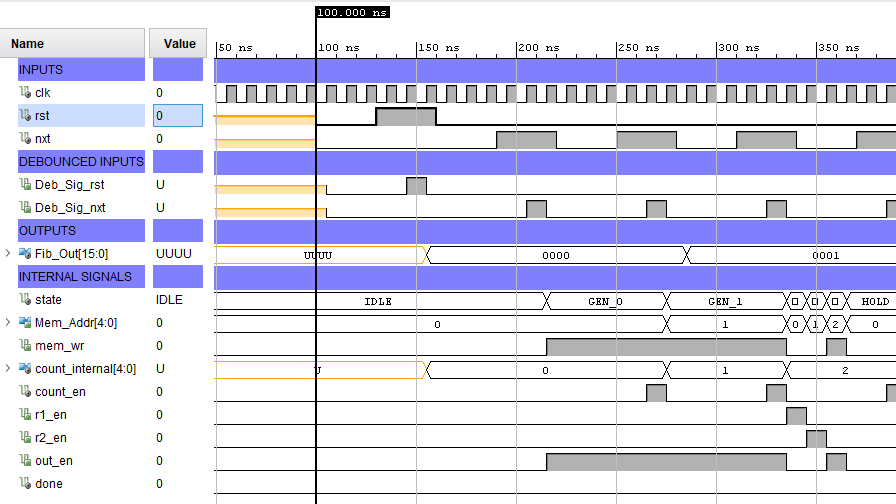
\includegraphics[width=0.9 \textwidth]{simulation_b_initial_reset.png}}
    \caption{Initialisation stage of the Fibonacci generator}
    \label{fig:simulation_b_initial_reset}
\end{figure}

\newpage

The timing diagram in \autoref{fig:simulation_b_normal_operation} shows the normal operation of the circuit. 
It can be seen that when a next state signal arrives during the HOLD state, the counter increments and the circuit transitions to the next state, which is LD\_R1 at which point the r1\_en (enable) signal is set to logic high. Then, on the next rising edge the controller automatically goes to the next state (LD\_R2) and the enable of the second register is triggered. Those two states load the last two numbers from the memory in order to generate the next one which happens at the state STORE. At this point, the memory write and the output enable are set to logic high. Finally the controller goes automatically into HOLD state and waits for next state input signal. 
\begin{figure}[ht]
    \centering
    \fbox{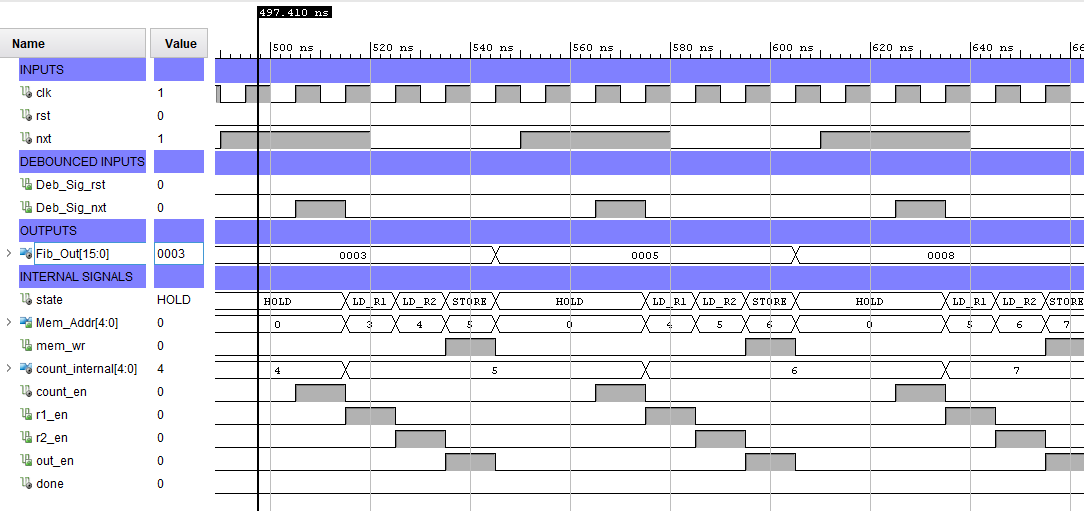
\includegraphics[width=0.9 \textwidth]{simulation_b_normal_operation.png}}
    \caption{Normal operation of the Fibonacci generator}
    \label{fig:simulation_b_normal_operation}
\end{figure}
\newpage

The timing diagram in \autoref{fig:sim_b_going_to_0} illustrates the roll-over point. When the counter reaches the value of 24, a "done" signal is generated, the highest Fibonacci number is created (0xB520, 46368 in decimal) and after the HOLD state, the controller goes back to state GEN\_0 and the sequence is repeated. 

\begin{figure}[ht]
    \centering
    \fbox{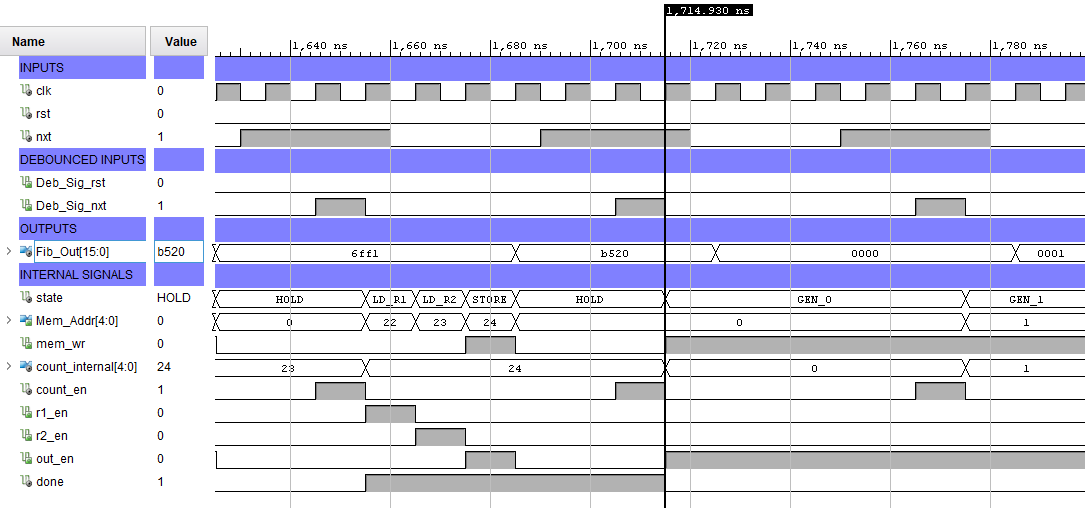
\includegraphics[width=0.9 \textwidth]{sim_b_going_to_0.png}}
    \caption{When Fibonacci sequence goes to 0}
    \label{fig:sim_b_going_to_0}
\end{figure}

The timing diagram in \autoref{fig:sim_b_reset} shows that the reset procedure operates successfully since the controller goes to IDLE state and the internal counter resets to 0.
\begin{figure}[ht]
    \centering
    \fbox{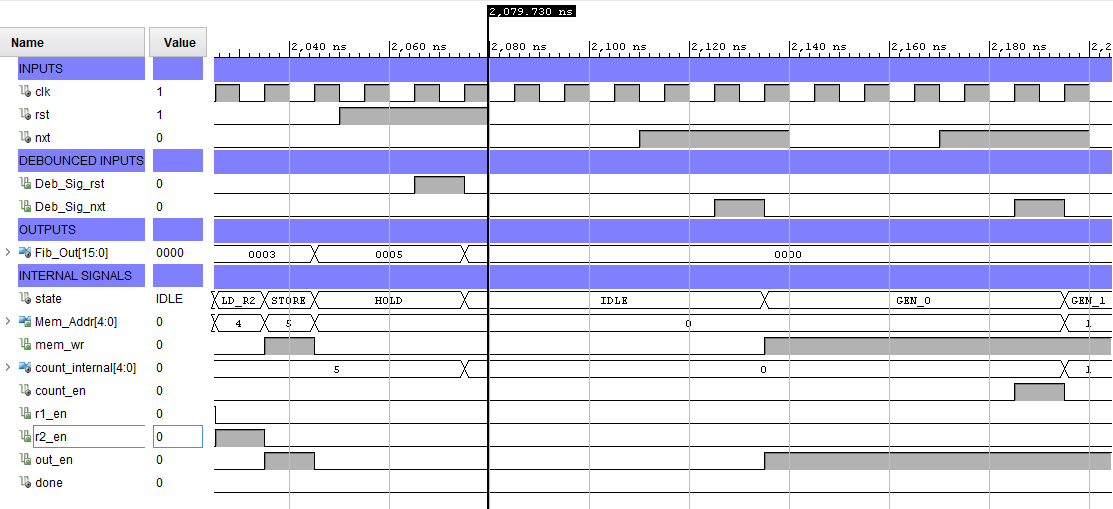
\includegraphics[width=0.9 \textwidth]{sim_b_reset.png}}
    \caption{Testing the reset functionality of the Fibonacci generator}
    \label{fig:sim_b_reset}
\end{figure}
\newpage

For completeness, a freeze and resume procedure was tested and illustrated in \autoref{fig:sim_b_freeze_resume}, to ensure that when the controller is in the HOLD state, the input clock has no effect if there are no present reset or next state signals.

\begin{figure}[ht]
    \centering
    \fbox{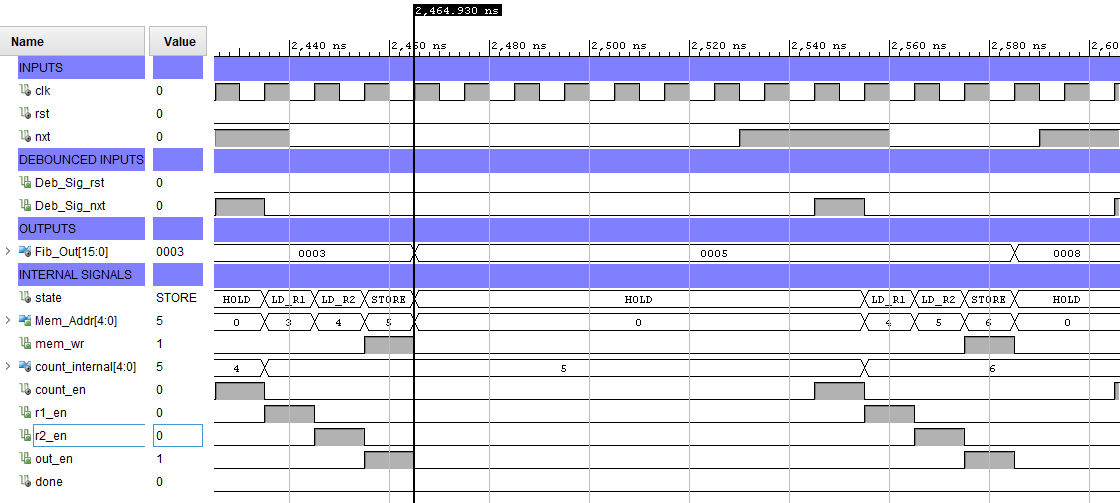
\includegraphics[width=0.9 \textwidth]{sim_b_freze_releze.png}}
    \caption{Freezing and resuming the Fibonacci generator}
    \label{fig:sim_b_freeze_resume}
\end{figure}
\newpage
\subsection {RTL Statistics}
In this section of the lab, the FSM-based Fibonacci generator was implemented successfully and displays as
expected in the state encoding table, the RTL component statistics and the RTL hierarchical component statistics.
\begin{minted}{text}
---------------------------------------------------------------------------------
        State |                 New Encoding |                Previous Encoding 
---------------------------------------------------------------------------------
         idle |                         000 |                              000
        gen_0 |                         001 |                              001
        gen_1 |                         010 |                              010
        ld_r1 |                         011 |                              011
        ld_r2 |                         100 |                              100
        store |                         101 |                              101
         hold |                         110 |                              110
---------------------------------------------------------------------------------
---------------------------------------------------------------------------------
Start RTL Component Statistics 
---------------------------------------------------------------------------------
Detailed RTL Component Info : 
+---Adders : 
	   2 Input     16 Bit       Adders := 1     
	   2 Input      5 Bit       Adders := 3     
+---Registers : 
	               16 Bit    Registers := 3     
	                5 Bit    Registers := 1     
	                1 Bit    Registers := 6     
+---Muxes : 
	   2 Input     16 Bit        Muxes := 2     
	   2 Input      5 Bit        Muxes := 2     
	   3 Input      5 Bit        Muxes := 1     
	   8 Input      3 Bit        Muxes := 1     
	   3 Input      2 Bit        Muxes := 1     
	   2 Input      1 Bit        Muxes := 3     
	   7 Input      1 Bit        Muxes := 1     
---------------------------------------------------------------------------------
Finished RTL Component Statistics 
---------------------------------------------------------------------------------
\end{minted}
\newpage
\begin{minted}{text}
---------------------------------------------------------------------------------
Start RTL Hierarchical Component Statistics 
---------------------------------------------------------------------------------
Hierarchical RTL Component report 
Module Debouncer 
Detailed RTL Component Info : 
+---Registers : 
	                1 Bit    Registers := 3     
Module Datapath 
Detailed RTL Component Info : 
+---Adders : 
	   2 Input     16 Bit       Adders := 1     
+---Registers : 
	               16 Bit    Registers := 3     
+---Muxes : 
	   2 Input     16 Bit        Muxes := 2     
Module Control 
Detailed RTL Component Info : 
+---Adders : 
	   2 Input      5 Bit       Adders := 3     
+---Registers : 
	                5 Bit    Registers := 1     
+---Muxes : 
	   2 Input      5 Bit        Muxes := 2     
	   3 Input      5 Bit        Muxes := 1     
	   8 Input      3 Bit        Muxes := 1     
	   3 Input      2 Bit        Muxes := 1     
	   2 Input      1 Bit        Muxes := 3     
	   7 Input      1 Bit        Muxes := 1     
---------------------------------------------------------------------------------
Finished RTL Hierarchical Component Statistics
---------------------------------------------------------------------------------
\end{minted}
\newpage

\subsection{Schematic}
 \autoref{fig:FSM_fibonacci_schematic} presents the top level schematic of the Fibonacci generator. In other words, all of the separate VHDL files that were included in Fibonacci.vhd are presented as their own components.
\begin{figure}[ht]
    \centering
    \fbox{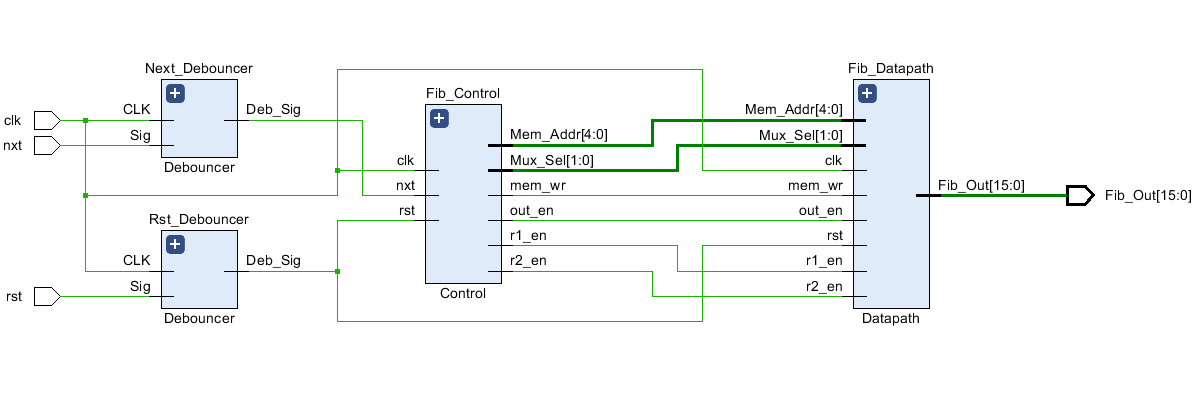
\includegraphics[width=0.9 \textwidth]{fibonacci_schematic_b.png}}
    \caption{Schematic of the FSM-based Fibonacci generator }
    \label{fig:FSM_fibonacci_schematic}
\end{figure}

The schematic in \autoref{fig:debounce schematic} exhibits the hardware implementation of the debounce circuit (Debouncer.vhd). The implementation uses three separate D-registers, also known as D-type flipflops, and an output word which collects the data of the outputs of those registers and produces the result of the debounce circuit. This is to be expected, because there were three separate internal STD\_LOGIC\_VECTOR lines in the VHDL file regarding that schematic.
\begin{figure}[ht]
    \centering
    \fbox{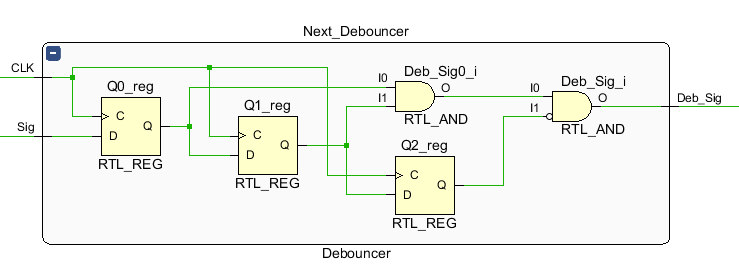
\includegraphics[width=0.9 \textwidth]{deb_schematic_b.png}}
    \caption{Schematic of a debouncer}
    \label{fig:debounce_schematic_B}
\end{figure}
\newpage

\autoref{fig:control_schematic_A} and \autoref{fig:control_schematic_B} present the schematic of Control.vhd. Although the schematic looks complex, at a closer inspection, it actually represents a coherent interpretation of the VHDL code. For instance in \autoref{fig:control_schematic_A} in the bottom left corner it could be seen the implementation of the counter process consisting of a register (count\_internal\_reg[4:0]) a multiplexer to spot the roll over value of 24, and an adder.
Also the transitions process is implemented in a similar manner. The register that stores the current state could be found in the bottom right counter of \autoref{fig:control_schematic_A}. The values used to represent the states could be seen in the state encoding table in Section 3.4. and that register has a feedback that goes into a multiplexer in the top right corner to select the value for the next state.
The same correspondence between the VHDL code and the schematic applies to the other components of the controller. 

\begin{figure}[ht]
    \centering
    \fbox{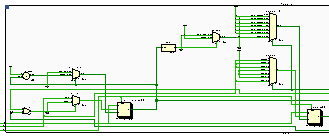
\includegraphics[width=0.9 \textwidth]{schematic-cropped1.pdf}}
    \caption{Schematic of the first part of the Fibonacci control logic}
    \label{fig:control_schematic_A}
\end{figure}


\begin{figure}[ht]
    \centering
    \fbox{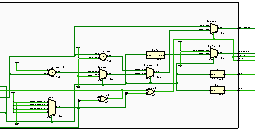
\includegraphics[width=0.9 \textwidth]{schematic-cropped2.pdf}}
    \caption{Schematic of the Second part of the Fibonacci control logic}
    \label{fig:control_schematic_B}
\end{figure}
\newpage
It is almost trivial to describe the relationship between the VHDL code and the schematic since the schematic seems to be a near identical representation of the VHDL code, with the only exception being that instead of a single multiplexer, as it is in the code, the schematic divides it into two.
\begin{figure}[ht]
    \centering
    \fbox{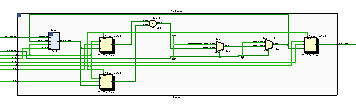
\includegraphics[width=0.9 \textwidth]{fib_datapath_schematic.pdf}}
    \caption{Schematic of the Fibonacci datapath module}
    \label{fig:datapath_schematic}
\end{figure}
\newpage

 \section{Conclusion}
 Both of the prescribed tasks were successfully implemented and tested. This lab clearly helped one understand how to implement digital circuits with memory and FSMs. It also revealed some easy to miss details when implementing digital systems and challenged one to think about the problems in an applicable manner.
 
 
 \newpage
 
\end{document}  